\documentclass[../main/main.tex]{subfiles}

\begin{document}

\newpage
\chapter{Evaluation}
Overall, I believe that my final program has effectively achieved the requirements set out by my client. It is a step-up to current alternatives that I have found online, and seems to be a solid choice for anyone wanting to play laser chess digitally.

\section{Objectives}
\subsection{Objective 1}
All laser chess game logic should be properly implemented. Refer to Figure \ref{fig:screenshots-game}.

Both the play and review screens display a 10x8 laser chess board. The laser fires automatically after every move, and follows the trajectory as directed by the pieces, destroying any that are facing the wrong way (Objectives \ref{obj:1f}, \ref{obj:1g}). All the pieces reflect and are destroyed by the laser correctly, with the colour to move alternating between both players (Objectives \ref{obj:1a}-\ref{obj:1e}). The game ends when a player either draws or resigns, has their pharaoh destroyed, or reaches three-fold repetition (Objectives \ref{obj:1h}, \ref{obj:1i}).

The game logic runs successfully, Objective 1 is fulfilled.

\subsection{Objective 2}
Game should process user input correctly. Refer to Figure \ref{fig:screenshots-game}.

Players can select, move and rotate pieces on their respective turns, through clicking squares, rotate buttons or by dragging the pieces (Objectives \ref{obj:2a}, \ref{obj:2c}, \ref{obj:2d}, \ref{obj:2e}). The game cancels any invalid moves (Objective \ref{obj:2b}). When a player holds down on a piece, the piece is moved through the drag-and-drop mechanism, and is released on the hovered square (Objective \ref{obj:2d}).

Objective 2 is fulfilled.

\subsection{Objective 3}
Save or load game options should be implemented. Refer to Figures \ref{fig:screenshots-browser} and \ref{fig:screenshots-review}.

In the browser screen, users can scroll through all previous games, with the option to delete or review them, or copy their FEN string (Objectives \ref{obj:3c}, \ref{obj:3f}, \ref{obj:3g}). Games can be sorted, and pages of games can be scrolled through (Objectives \ref{obj:3d}, \ref{obj:3e}). The game positions are encoded using a custom FEN string format, and games are saved as rows in a local SQLite database table (Objectives \ref{obj:3a}, \ref{obj:3b}). In the review screen, users can scroll through all the moves of a previous game (Objective \ref{obj:3i}). The right sidebar displays information such as the winner and move number, and the timer, pieces and move list updates accordingly (Objective \ref{obj:3h}).

Objective 3 is fulfilled. A possible improvement would be to add the option of loading up a position to resume playing straight from the review screen. This would be a convenient feature, but is not a priority, as users can currently copy the FEN string from the browser screen to the config screen and load the position there as a current alternative.

\subsection{Objective 4}
Other board game requirements should be implemented. Refer to Figure \ref{fig:screenshots-game}.

In addition to the core game mechanics, other ancillary aspects are added as well. Timers can be enabled and disabled, decrement correctly, and end the game when they run out (Objectives \ref{obj:4c}, \ref{obj:4d}). Buttons also exist for drawing and resigning the game (Objectives \ref{obj:4a}, \ref{obj:4b}).

Objective 4 is fulfilled.

\subsection{Objective 5}
Game settings and config should be customisable. Refer to Figures \ref{fig:screenshots-settings} and \ref{fig:screenshots-config} and \ref{fig:screenshots-editor}.

In the settings screen, the user can change settings to toggle the volume, fullscreen, board colours, particles and shaders (Objectives \ref{obj:5i}, \ref{obj:5j}). All settings update correctly, and are saved to a local JSON file when the settings screen is exited. The game configurations are changed in the config screen. Here, users can change the game's starting colour, configure timer settings, change to the CPU player and specify the difficulty, select a board preset, or create a custom board layout through the editor screen (Objectives \ref{obj:5a}-\ref{obj:5c}). The editor screen comes with all the basic operations of placing pieces, rotating pieces, and erasing and dragging them, but also helpful buttons to erase or reset the board (Objectives \ref{obj:5f}-\ref{obj:5h}). Another method to change the board layout is through inputting a FEN string, and the board either updates or displays an error message depending on the validity of the string (Objectives \ref{obj:5d}, \ref{obj:5e}).

Objective 5 is fulfilled.

\subsection{Objective 6}
Game UI should improve player experience. Refer to Figure \ref{fig:screenshots-game}.

Indicators are present to highlight the selected square and any adjacent squares that it can be moved to (Objectives \ref{obj:6a}, \ref{obj:6b}). Audio cues also improve the immersiveness of the game, as well as the laser visuals and particle effects (Objective \ref{obj:6c}). The mouse cursor was also modified to help user-friendliness, by changing its icon depending on the current action being performed, for example, a closed hand icon for grabbing a piece (Objective \ref{obj:6g}). The move list and status message widgets are positioned on the right of the game screen, update accordingly and provide information on the game (Objectives \ref{obj:6e}, \ref{obj:6f}). The piece display also correctly updates to show all destroyed pieces (Objective \ref{obj:6d}).

Objective 6 is fulfilled.

\subsection{Objective 7}
GUI design should be functional and display concise information. Refer to Figure \ref{fig:screenshots-menu}.

I have created most of the custom pixel art and icon graphics to improve the game's visual and attempt to make it more engaging (Objective \ref{obj:7c}) There are currently 7 screens in the game: menu, settings, config, editor, game, browser and review, each containing their own eponymous function (Objective \ref{obj:7b}). Most screens also contain both the main menu button and help button. Clicking the menu button switches to the main menu screen, and clicking the help button shows an overlay displaying the functionality of drawn widgets (Objective \ref{obj:7d}). Shaders are also used to improve the game's visuals, such as by giving the laser a light-emitting effect, but is also used to draw all the backgrounds (Objective \ref{obj:7e}). The program runs well, with moments involving heavy calculation being helped by multithreading, and also resizes seamlessly (Objective \ref{obj:7a}, \ref{obj:7f}).

Objective 7 is fulfilled. Working on Windows, I did not bundle the program to macOS or Linux. Although this was not a priority, having access to other OS testing environments would've widened access to the game.

\section{Client Feedback}
An interview was conducted after Mr Myslov received and played through the program, the following transcription is summarised and paraphrased for clarity.

\begin{figure}[H]
    \centering

    \begin{subfigure}[b]{0.49\columnwidth}
    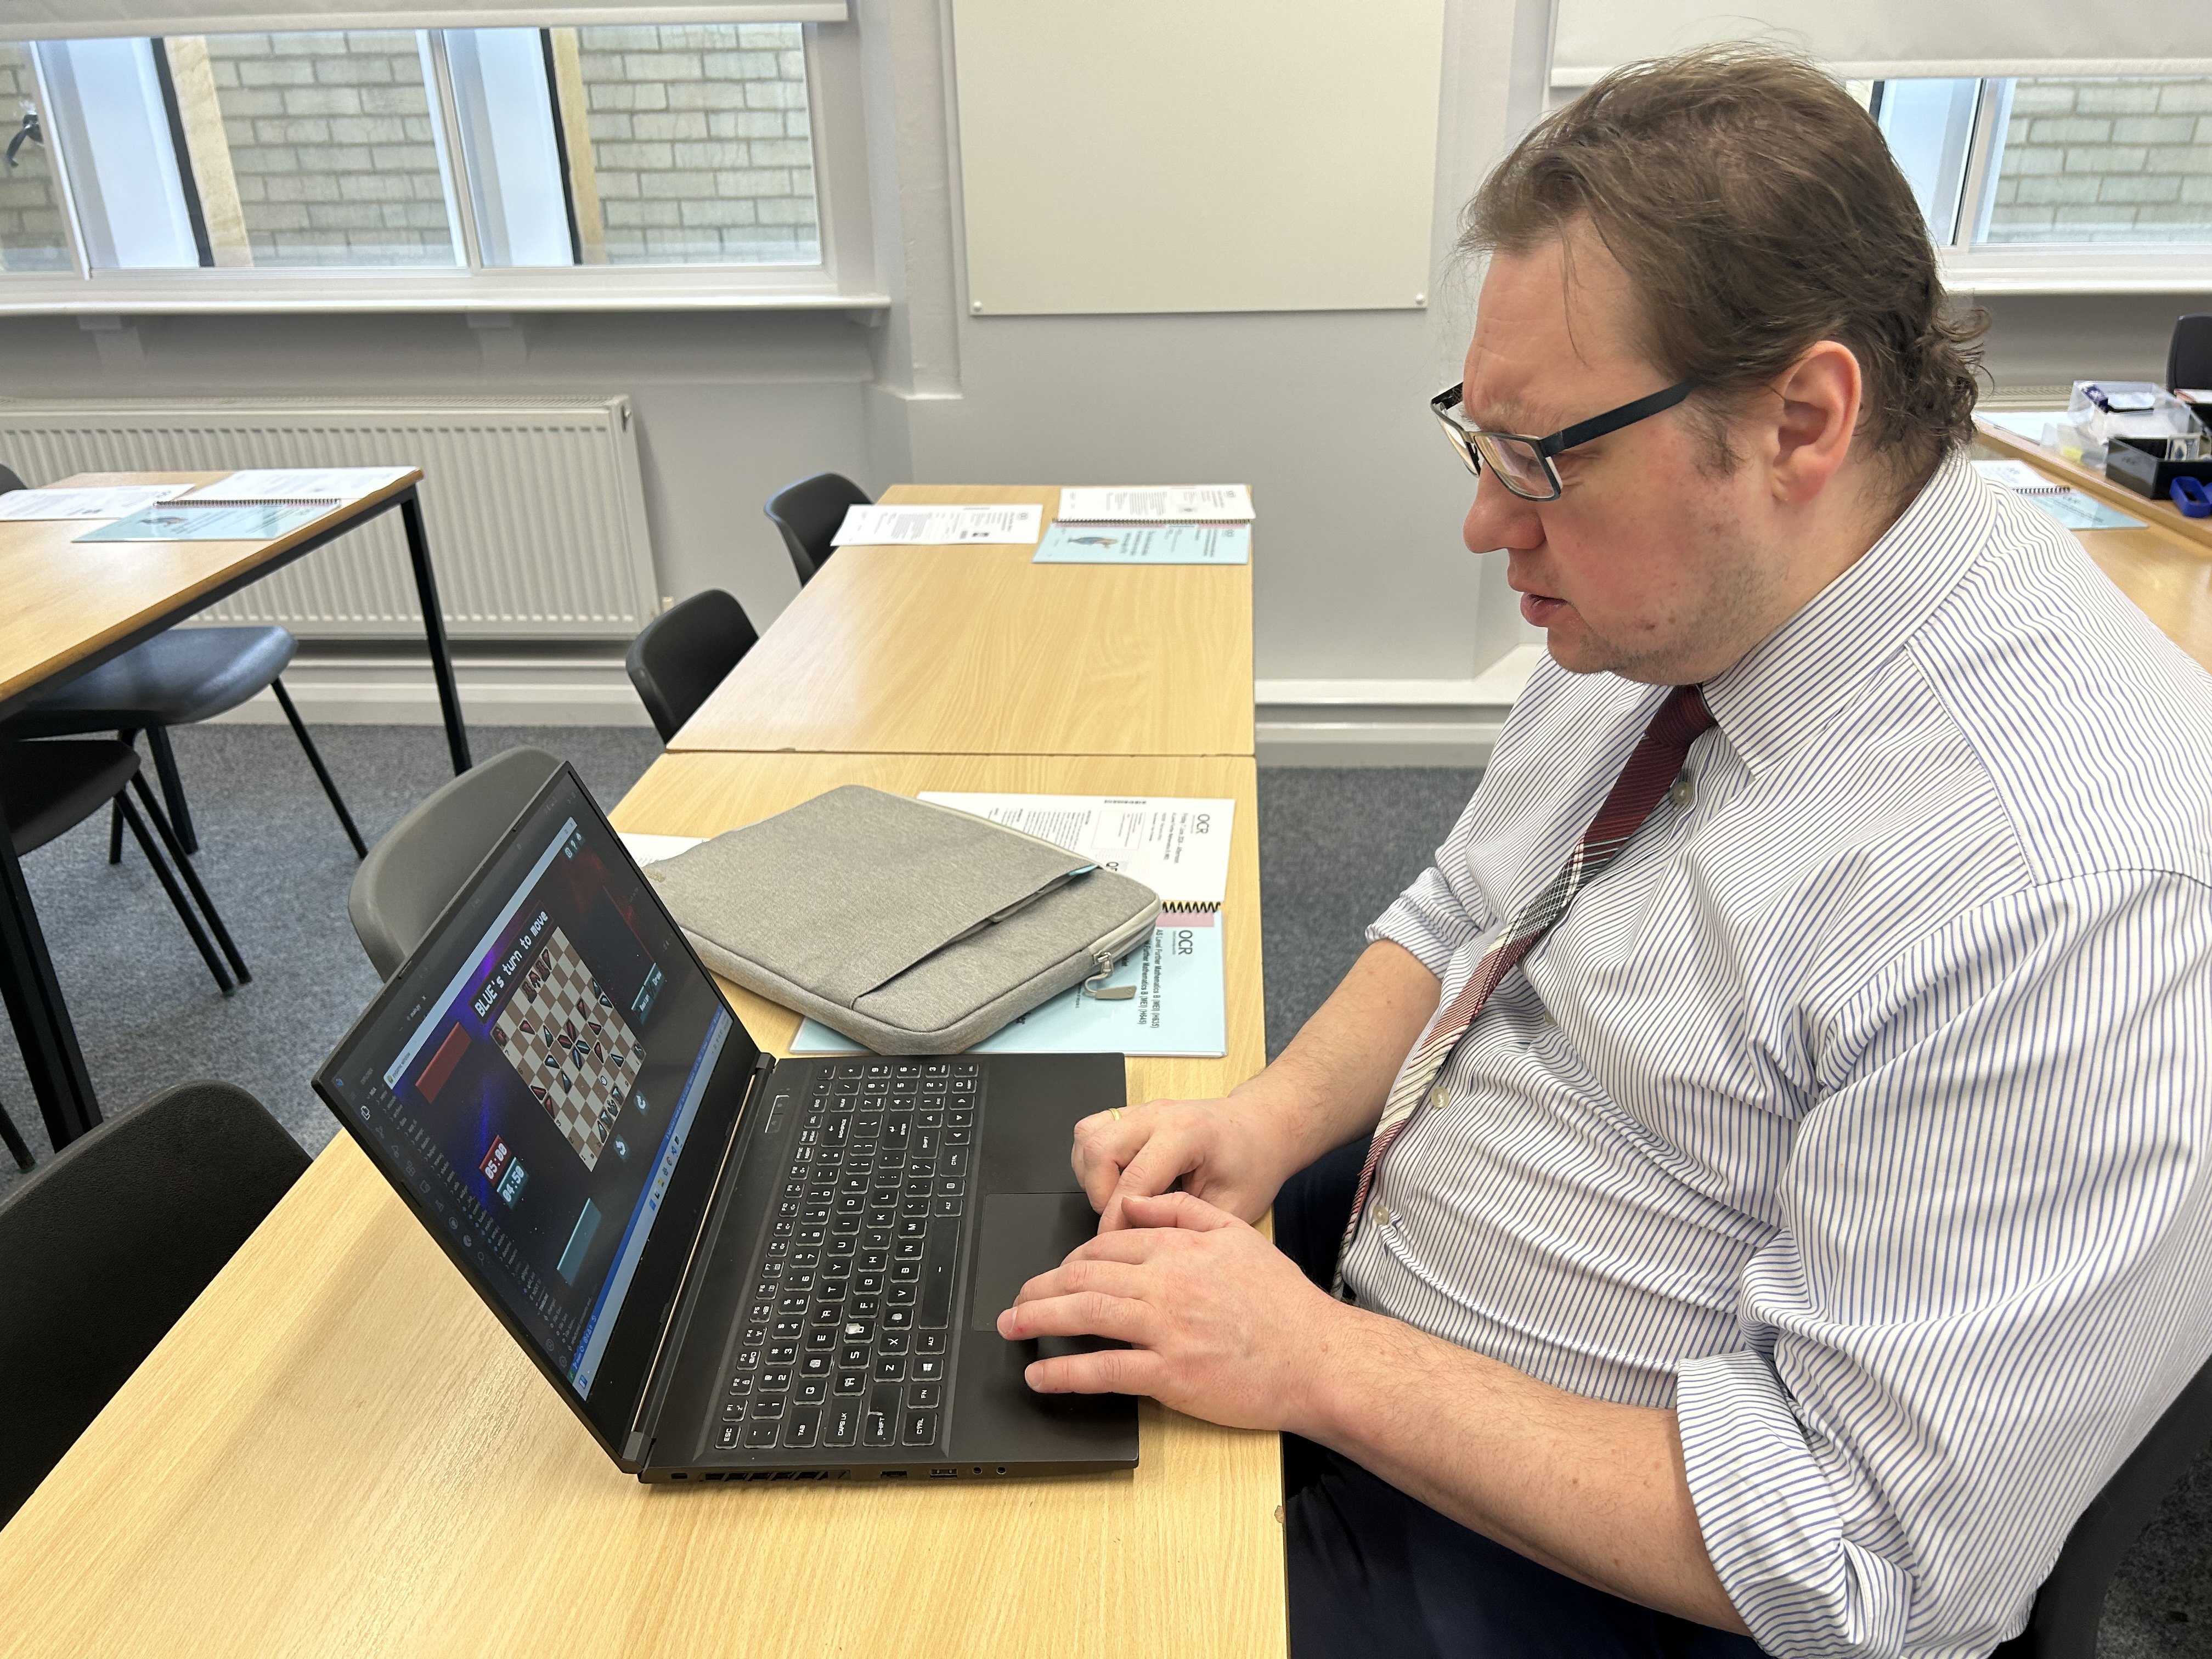
\includegraphics[width=\columnwidth]{../evaluation/assets/myslov_playing.jpeg}
    \end{subfigure}
    \hfill
    \begin{subfigure}[b]{0.49\columnwidth}
    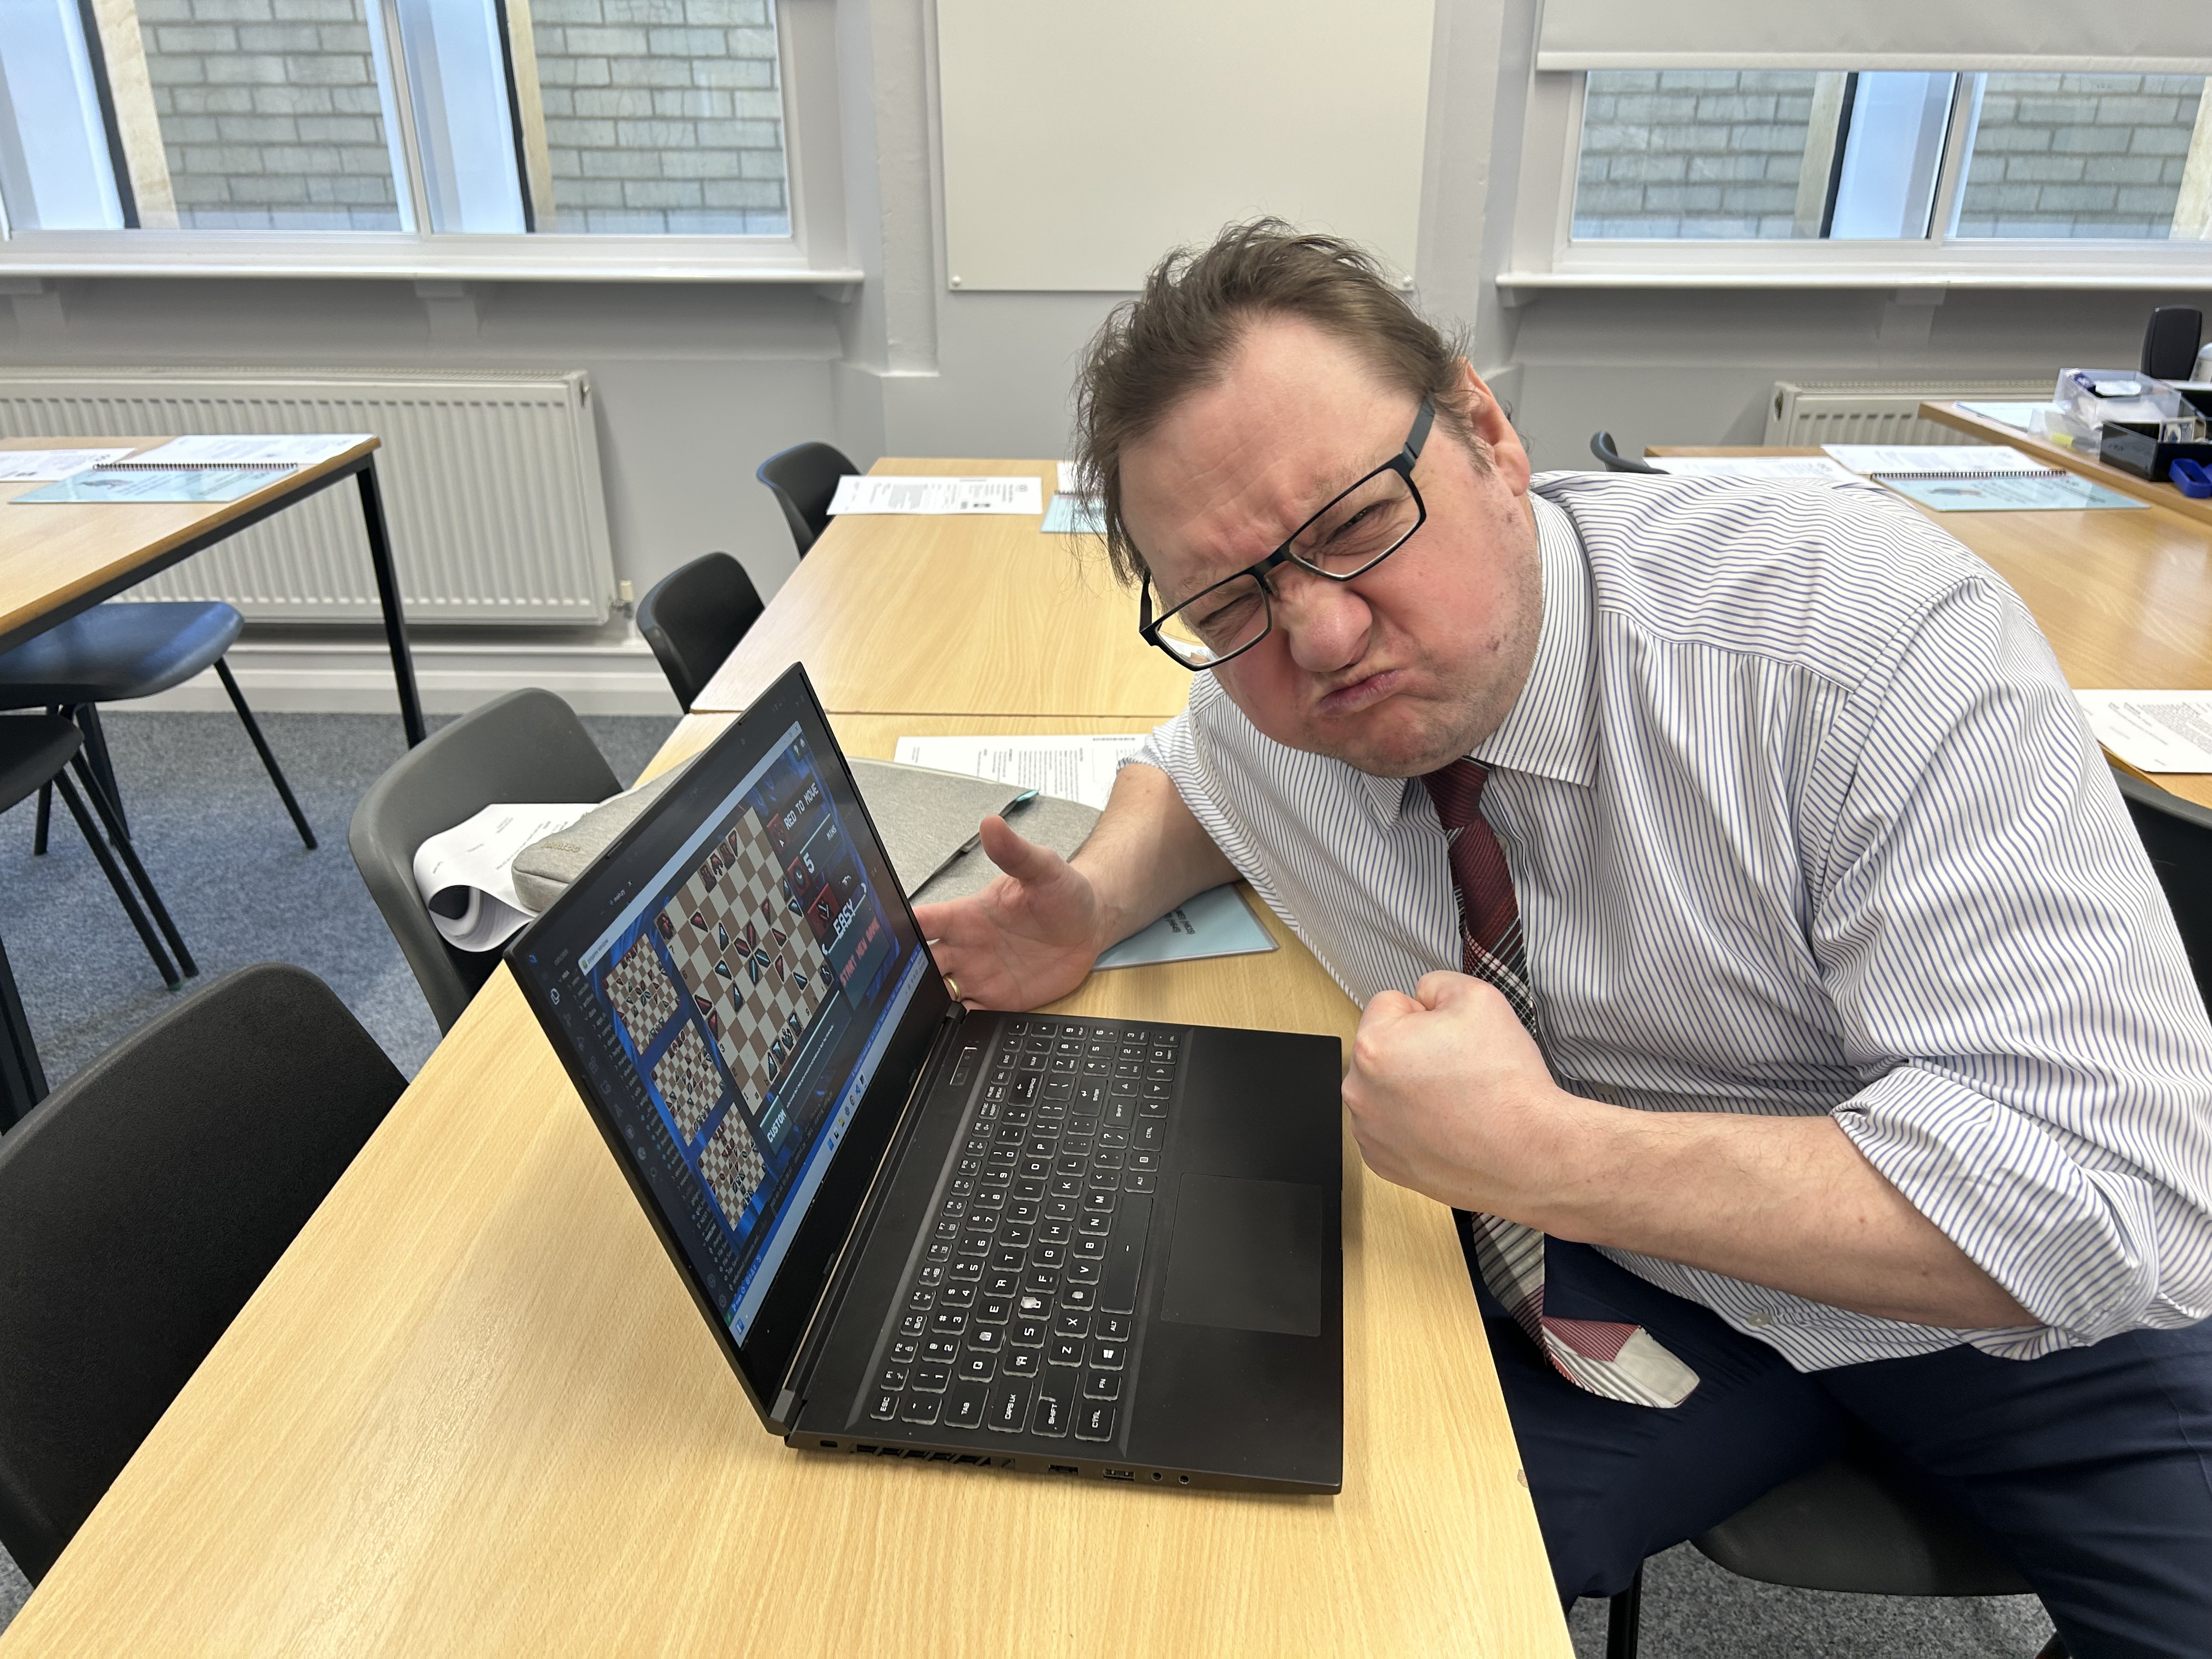
\includegraphics[width=\columnwidth]{../evaluation/assets/myslov_angry.jpeg}
    \end{subfigure}

\caption{(left) Mr Myslov playing through the game (right) Mr Myslov physically threatens me after failing to beat the bot}
\label{fig:client-interview}
\end{figure}

\noindent\textbf{Q:} Did the final product meet your expectations?

\noindent\textbf{A:} Yes, it certainly did. The game plays perfectly, I could move, rotate all the pieces as expected, and the laser works well. All the features I requested for were there, and I also like your indie-style graphics.

\noindent\rule{\textwidth}{0.4pt}

\noindent\textbf{Q:} What improvements could be made to the program?

\noindent\textbf{A:} There seems to be quite a steep learning curve towards your program. It was hard understanding how the pieces worked with the laser. Playing through the game the CPU was also initially difficult, especially on the easy difficulty, as the moves would be played instantly after I moved, and I wasn't sure what move was made or whether the laser fired before or after my move. The bot was also frustrating to play against as it is very defensive, so I couldn't capture any of its pieces, it needs to be dumber; I don't know if the bot is intended to accept my draw, but I think that's good. I also like that you have made your own FEN string implementation confusing, but I'm not too sure how it works or what the characters mean.

\noindent\rule{\textwidth}{0.4pt}

\noindent\textbf{Q:} What other aspects would you like to have been added?

\noindent\textbf{A:} Being able to somehow easily obtain a digital file for a game would be useful, so I could share it with my students easily. To help with learning the game, you could add some puzzles to help with solving tactics and getting used to the pieces, and also a highlight overlay for moves played because it was hard to follow or figure out.

\subsection*{Discussion}
My client was satisfied with my final program. His perspective revealed some aspects of the program that could've better considered and improved upon. Mr Myslov also helped discover a bug when he tried to offer a draw to the bot, who instantly accepted it despite being in a winning position. He seemed to enjoy this unexpected outcome, so I will consider this a feature.

\paragraph{User-friendliness} was the core discussion point raised by Mr Myslov. He highlighted the fact that it would be hard for beginners to understand the rules of laser chess, which I agree on, considering that the rules and pieces are very different from regular chess.  To amend this, I could add more tutorials or puzzles as per suggested, for instance, by creating a new tutorial or puzzle screen containing a miniaturised board, where the user can learn how the pieces interact with the laser; although a help screen is already implemented, an interactive one would perhaps serve the purpose more efficiently. A similar approach could be applied to my custom FEN string and algebraic move notation.

\paragraph{Sharing games} was a suggestion made by Mr Myslov. Although the FEN string system allows for sharing of board positions, I realise that there is value in also sharing the entire progression of the game. This could be implemented by exporting the game to the equivalent of a chess 'PGN' file, by writing all the game information (e.g. CPU depth) to a .txt file, and then the contents of the move list.

\paragraph{CPU} was also another point to consider. Mr Myslov complained that the CPU's thinking time on the easy mode was too short, resulting in his opponent's move being played instantly, confusing the flow of the game and making it hard to see what move was made. To fix this, I could either increase the thinking time artificially for the easy setting by only applying the move after a set timer runs out, or add an overlay similar to the one for selecting pieces, over the squares that a moved piece was on and has moved to. Mr Myslov also complained about the CPU's defensive style and his inability to gain an advantage. Although this can be regarded as a compliment, I agree that the CPU's tendency to defend instead of attack can be annoying. This results from the relative weighing of the evaluation function, which could be updated to contain PSQTs giving higher scores for more aggressive piece positioning, reducing the score allocated for king safety, or adjusting the piece values for a more aggressive play style.

\bigskip

\noindent Regardless, given the limited time frame, we were both pleased with the final result.s

\section{Further improvements}
There are some improvements that I have considered that were not brought up in the objectives or in interview.

A point not raised by Mr Myslov was the ease-of-use of the widgets. The one that I found concerning was the text input, as constantly deleting the entire FEN string, and having to manually press arrow keys to edit specific characters was tedious. I have tried to improve this by adding shortcuts such as \verb|Ctrl+Backspace| to delete the entire contents of the text Input. To improve the text input to make it feel more familiar to standard ones, I would have to use two pointers to track the indexes of the start and end characters, for the ability to highlight and delete chunks of text. The text displayed can also be hard to read currently, especially if there are a lot of characters. This could be improved by either fixing the font width, detecting if the text width is greater the widget width and implementing text wrapping, or allowing text scrolling.

Multiplayer was another improvement suggested by Mr Myslov. Admittedly, this is a big feature for a digital board game, however, I did not implement this as it was not a requested objective, and would've required restructuring my code for handling moves and the game logic. This could be achieved within Python through a peer-to-peer system, sending and parsing formatted moves either through pickling or JSON objects via HTTP methods using the \lstinline{requests} module, although it would also require an overhaul of the GUI and screens to allow the option for multiplayer.

Performance issues did not appear throughout Mr Myslov's playthrough. However, even if the program runs smoothly on my device, some fragment shaders are computationally expensive and may affect the performance on other devices. I have attempted to resolve this by adding the option to disable shaders, however, a better solution would be to optimise the expensive shader code, for example, by approximating masks using widget dimensions instead of the in-built pixel perfect Pygame mask function.

\section{Conclusion}
The final product fulfilled all proposed objectives and more, and has been approved by my client.

Throughout 6 months of development, I felt that I improved on many aspects needed to be a proficient developer. Creating bespoke software allowed for conducting research, interviews, and also obtaining continuous feedback. In terms of coding, working on a large project helped in improving file management, documentation, and keeping robust backups through Git. It also gave me the opportunity to learn GLSL for my shaders, LibreSprite for pixel art, and LaTeX for my documentation. Having a greater familiarity with Pygame, I also plan to rework my widget system as a library, to be shared for the benefit of all future Pygame users.

Overall, this project was a success.

\end{document}